\documentclass[12pt]{article}
{\usepackage{amsmath,amssymb,amsthm,enumerate,dsfont,bm}
\usepackage{pdfpages}
\usepackage[a4paper,bindingoffset=0.2in,%
left=0.8in,right=0.8in,top=1in,bottom=1in,%
footskip=.25in]{geometry}

\newcommand{\prob}[1]{\textbf{P}(#1)}
\newcommand{\ep}[1]{\mathbb{E}\left[ #1 \right]}
\newcommand{\var}[1]{var \left( #1 \right)}
\newcommand{\cp}{\overset{p}{\to}}
\newcommand{\cas}{\overset{a.s.}{\to}}
\newcommand{\cd}{\overset{D}{\to}}

\title{Statistical Theory Homework 5}
\date{\today}
\author{Bohao Tang}

\begin{document}
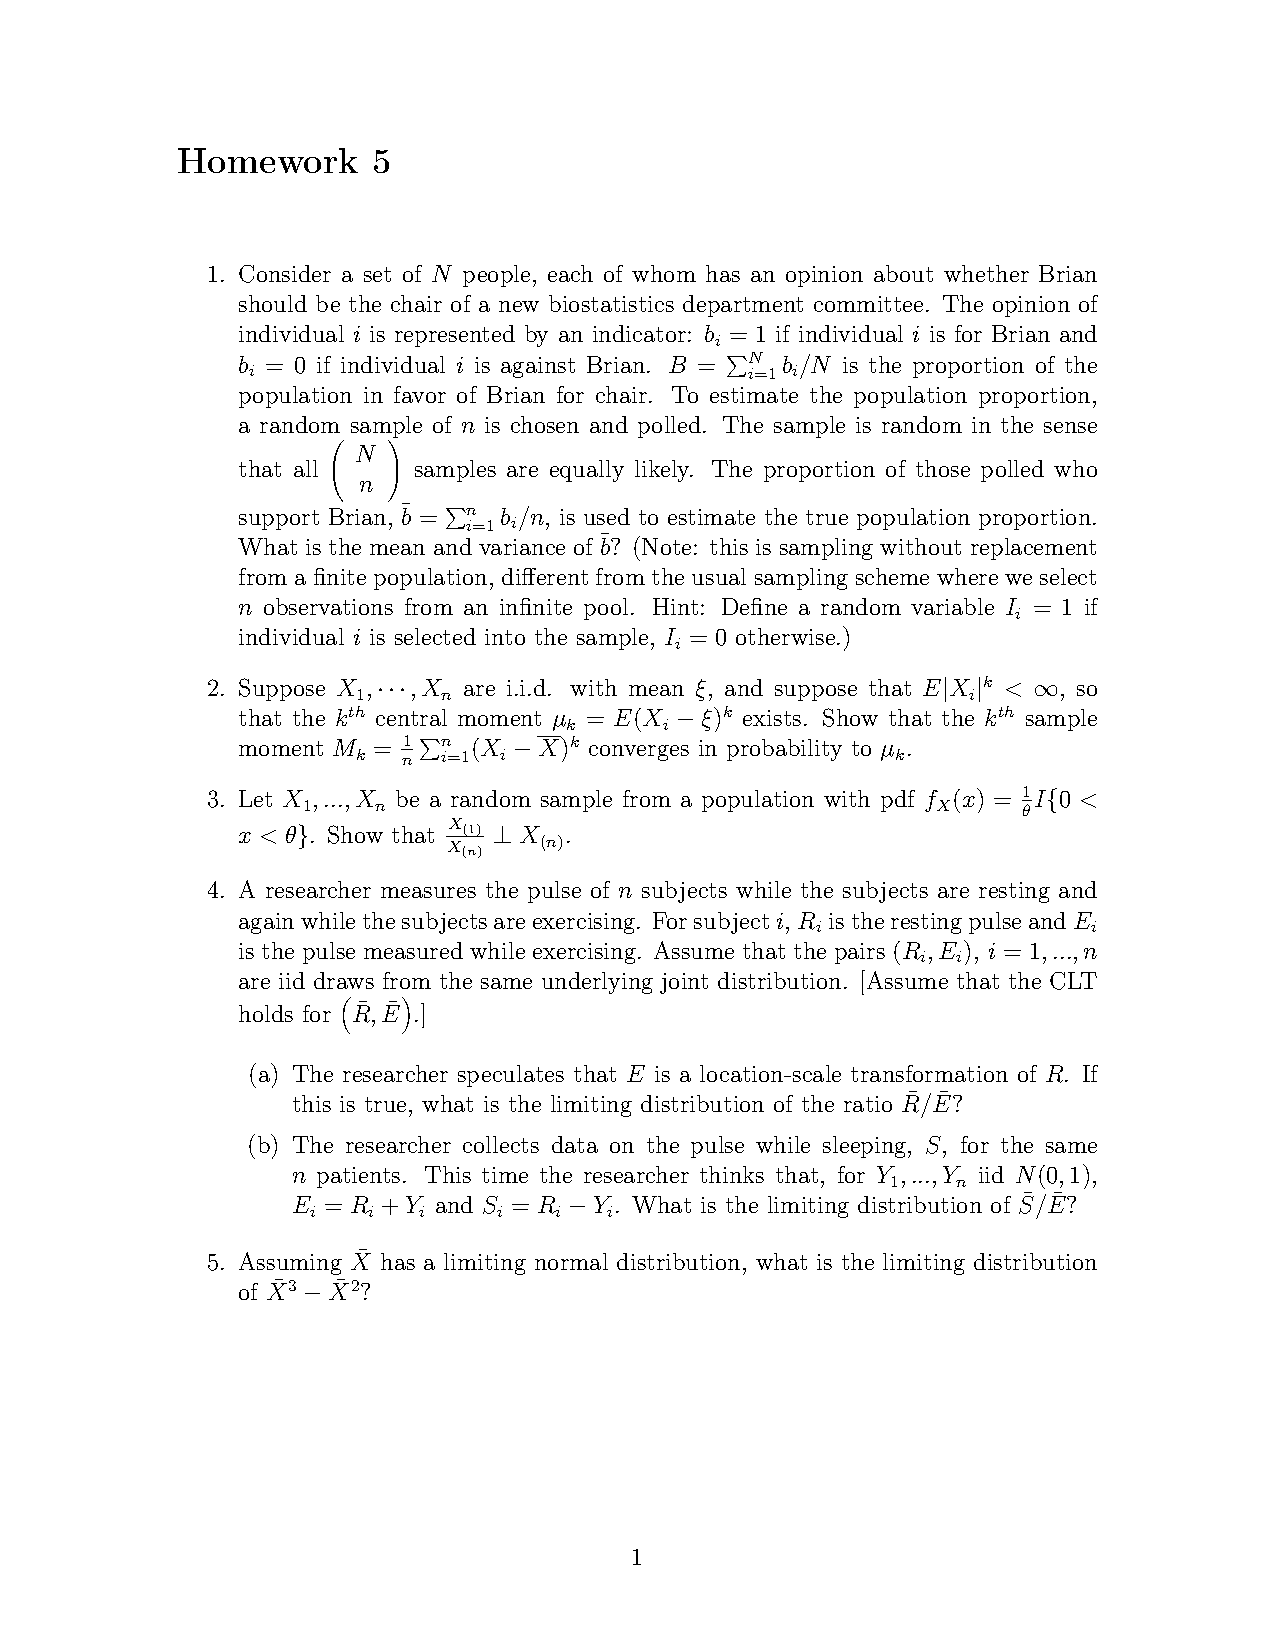
\includepdf[pages=-]{HW_5.pdf}
\maketitle

\begin{enumerate}
    \item 
    Here $B, N, n$ are all known. Define random variables $I_i$: $I_i = 1$ if individual $i$ is selected into bthe sample and $I_i = 0$ otherwise.
    
    $N$ should be large, or we don't need to choose a sample, and the sample number should be reasonable large. So we here don't consider the extreme condition with $N \le 2$ or $n \le 2$. We suppose $N > 2$ and $n > 2$. 

    Then we have that $\bar{b} = \frac{\sum_{i=1}^N b_i I_i}{n}$. Therefore:
    $$\ep{\bar{b}} = \frac{1}{n} \sum_{i=1}^N b_i \ep{I_i} = \frac{1}{n} \sum_{i=1}^N \frac{n b_i}{N} = B$$
    And
    \begin{eqnarray}
        \var{\bar{b}} &=& \ep{\bar{b}^2} - \ep{\bar{b}}^2 = \frac{1}{n^2} \sum_{i,j}^{N} b_i b_j \ep{I_i I_j} - B^2 \\
                      &=& \frac{1}{n^2} \sum_{i \ne j}^N b_i b_j \frac{\binom{N-2}{n-2}}{\binom{N}{n}} + \frac{1}{n^2} \sum_{i}^N \frac{n b_i^2}{N} - B^2 \\
                      &=& \frac{1}{N} \frac{n}{N} \frac{n-1}{N-1} (\sum_{i,j}^N b_i b_j - \sum_i^N b_i^2) + \frac{B}{n} - B^2 \\
                      &=& \frac{(n-1) (N B^2 - B)}{n (N-1)} + \frac{B - n B^2}{n} \\
                      &=& \frac{(N-n)B(1-B)}{n(N-1)}
    \end{eqnarray} 

    \item
    \begin{proof}
    Suppose $k$ is a real number bigger than $1$, then by mean value theorem: 
    \begin{eqnarray}
        |(X_i - \bar{X})^k - (X_i - \xi)^k| &\le& |\xi - \bar{X}| | \max_{t \ \text{between} \ X_i-\bar{X}, X_i-\xi} k t^{k-1} | \\        
                                            &\le& |\xi - \bar{X}| k (|X_i - \bar{X}|^{k-1} + |X_i - \xi|^{k-1}) \\
                                            &\le& |\xi - \bar{X}| k \max(1,2^{k-2}) (2 |X_i|^{k-1} + |\bar{X}|^{k-1} + |\xi|^{k-1})
    \end{eqnarray}
    Here we use the $C_r$ inequality: $|a+b|^r \le \max(1,2^{r-1})(|a|^r + |b|^r)$ for $a,b \in \mathbb{R}$ and $r > 0$.
    Set $C = k \max(1, 2^{k-2})$, then we have:
    \begin{eqnarray}
        (\frac{1}{n}\sum_{i=1}^n (X_i - \bar{X})^k &-& \frac{1}{n}\sum_{i=1}^n (X_i - \xi)^k) \le |\frac{1}{n}\sum_{i=1}^n (X_i - \bar{X})^k - \frac{1}{n}\sum_{i=1}^n (X_i - \xi)^k| \\
                                                                                            &\le& \frac{1}{n} \sum_{i=1}^n |(X_i - \bar{X})^k - (X_i - \xi)^k| \\
                                                                                            &\le& C |\bar{X} - \xi| (|\xi|^{k-1}+|\bar{X}|^{k-1}+2\frac{\sum_{i=1}^n|X_i|^{k-1}}{n})    
    \end{eqnarray}
    Since $\ep{|X|^k} < \infty$, by H\"{o}lder inequality, we have $\ep{|X|^{k-1}} < \infty$. Therefore we have $\frac{\sum_{i=1}^n|X_i|^{k-1}}{n} \cp \text{Ma}_{k-1} = \ep{|X|^{k-1}}$. By continuous mapping theory, we have:
    \begin{eqnarray}
        &&|\bar{X} - \xi| \cp 0 \\
        &&(|\xi|^{k-1}+|\bar{X}|^{k-1}+2\frac{\sum_{i=1}^n|X_i|^{k-1}}{n}) \cp \text{constant..}
    \end{eqnarray}
    By Slutsky Theorem (notice that when convergent to a constant, converge in probability is equvilant to converge in distribution), we have $C |\bar{X} - \xi| (|\xi|^{k-1}+|\bar{X}|^{k-1}+2\frac{\sum_{i=1}^n|X_i|^{k-1}}{n}) \cp 0$.
    And then by definition $\frac{1}{n}\sum_{i=1}^n (X_i - \bar{X})^k - \frac{1}{n}\sum_{i=1}^n (X_i - \xi)^k \cp 0$. Together with $\frac{1}{n}\sum_{i=1}^n (X_i - \xi)^k \cp \mu_k$(weak law of large number) and Slutsky Theorem, we have that $\frac{1}{n}\sum_{i=1}^n (X_i - \bar{X})^k \cp \mu_k$.    
    \end{proof}

    \item
    \begin{proof}
        First, we write out the joint pdf of $X_{(1)}, X_{(n)}$: 
        $$f_{X_{(1)}, X_{(n)}}(x_1, x_n) = n(n-1)\frac{(x_n-x_1)^{n-2}}{\theta^n} \bm{1}_{0<x_1\le x_2<\theta}$$
        And then we do the transform $U = \frac{X_{(1)}}{X_{(n)}}; \  V = X_{(n)}$. We have $X_{(1)} = U V$, $X_{(n)} = V$ and $|\frac{\partial (X_{(1)},X_{(n)})}{\partial (U, V)}| = V$.
        So that the joint pdf of $U, V$ is:
        $$f_{U,V}(u,v) = \frac{n}{\theta^n} v^{n-1}\bm{1}_{0<v<\theta} \times (n-1)(1-u)^{n-2} \bm{1}_{0<u<1} $$
        Notice that $f_{U,V}$ can be factorized in production of function of $u$ and $v$. Therefore $U \bot V$, which means $\frac{X_{(1)}}{X_{(n)}} \bot X_{(n)}$. 
    \end{proof}
    
    \item
    \begin{enumerate}[(a)]
        \item
        Here, we have $E = a R + b$ for some constant $a>0,b$.(For specific $a = \sqrt{\frac{\var{E}}{\var{R}}}$ and $b = \ep{E} - a\ep{R}$) Suppose $\ep{R} = R_e$ and $\var{R} = \sigma^2$(of course $aR_e + b$ will not be zero !!).
        Then we have $\frac{\bar{R}}{\bar{E}} = \frac{\bar{R}}{a\bar{R} + b}$. By delta method, we have $\sqrt{n}(\frac{\bar{R}}{\bar{E}} - \frac{R_e}{aR_e + b}) = \sqrt{n}(\frac{\bar{R}}{a\bar{R} + b} - \frac{R_e}{aR_e + b}) \cd N(0, \sigma^2 \frac{b^2}{(aR_e+b)^4})$.
        \item
        Suppose $\ep{R} = R_e$, $var(R) = \sigma^2$ and $cov(R, Y) = \rho \sigma$. Then by CLT, we have $\sqrt{n}[(\bar{R},\bar{Y}) - (R_e,0)] \cd N(0, \begin{pmatrix}
                                                                                                                                                            \sigma^2 & \rho \sigma \\
                                                                                                                                                            \rho \sigma & 1                
                                                                                                                                                            \end{pmatrix})$.

        Therefore by delta method, we have:
        \begin{eqnarray}
            \sqrt{n}(\frac{\bar{S}}{\bar{E}} - 1) &=& \sqrt{n}(\frac{\bar{R} - \bar{Y}}{\bar{R} + \bar{Y}} - \frac{R_e - 0}{R_e + 0}) \\
            &&\cd N(0, \begin{pmatrix} 0 & -2/R_e \end{pmatrix} \begin{pmatrix}
            \sigma^2 & \rho \sigma \\
            \rho \sigma & 1                
            \end{pmatrix} \begin{pmatrix} 0 \\ -2/R_e \end{pmatrix})  \\
            &&\cd N(0, \frac{4}{R_e^2})
        \end{eqnarray}
    \end{enumerate}

    \item
    Suppose $\sqrt{n} (\bar{X} - \mu) \cd N(0,\sigma^2)$. Then by delta method, we have that $(x^3-x^2)'(\mu) = \mu(3\mu-2)$ and:
    $$\sqrt{n} [(\bar{X}^3 - \bar{X}^2) - (\mu^3 - \mu^2)] \cd N(0,\sigma^2 \mu^2 (3\mu -2)^2 )$$
\end{enumerate}
    
\end{document}